%!TEX root = umthsmpl.tex
\chapter{Graphene: Efficient Block Announcements}
\label{graphene}

In this chapter, we explain Graphene, a novel protocol for the propagation of blocks and status reports. The main limitation we are addressing with Graphene is the inefficiency of blockchain systems in propagating block data.  A block announcement must be validated using  the transaction content comprising the block.  However, it is likely that the majority of the peers have already received these transactions, and they only need to discern them from those in their mempool. Additionally, in Section~\ref{section:difficulty-proposed-work}, we propose using status reports (i.e., blocks announcements that do not satisfy the difficulty requirement of the network) for the emergency difficulty algorithm. Therefore, on top standard blocks, we are proposing to add more network traffic, requiring an even more efficient method of block propagation.

\section{Background}
In this subsection, we describe the signaling mechanism behind blockchain systems, explain the operation of Invertible Bloom Lookup Tables and summarize related work.

%%%%%%%%%%%%%%%%%%%%%%%%%%%%%%%%%%%%%%%%%%%%%%%
\subsection{Topology and Signaling in Blockchain Systems} 
Bitcoin Core propagates new transaction and
block announcements by flooding throughout a p2p random graph of full
nodes and miners. Each peer in the graph requests direct connections
to 8 other peers, and accepts requests for connections from up to 117
other peers. A peer will offer a newly created transaction to each
neighbor via an {\tt inv} message, which reports the hash of the
transaction content as its ID. If a peer does not already possess the
transaction, it will request it using a {\tt getdata} message. Blocks
are handled similarly: {\tt inv} messages describe a block by its ID, which
is created from the hash of the block's contents.  Upon receiving the
{\tt inv}, peers will request the block if they do not already have it.
Hence, in today's topology, {\tt inv} messages cross every edge in the
random graph once, while the actual transaction and block data
typically propagate along only a spanning tree of the graph (more
edges will be traversed if there are propagation delays).  For
convenience, we refer to the set of (unconfirmed)
transaction IDs that a peer knows about as the {\em IDpool}. Actual
transaction contents are placed in the mempool.

%%%%%%%%%%%%%%%%%%%%%%%%%%%%%%%%%%%%%%%%%%%%%%%
\subsection{Related Work} 
In principle, a block announcement needs to include only the IDs of those transactions,
and accordingly, Corallo's {\em Compact Block} design~\cite{Corallo:2016} --- which has been recently deployed --- significantly reduces block size by including a  transaction ID list at the cost of increasing coordination to 3 roundtrip times.
%After the block's {\tt inv} has been sent, the receiver requests the block. The sender sends the IDs of transactions (in fact, just the first 5 bytes of each). The receiver then requests the contents of any transaction if previously unseen.
%
{\em Xtreme Thinblocks}~\cite{Tschipper:2016}, an alternative protocol, works similarly to Compact Blocks but has greater data overhead. Specifically, Xtreme Thinblocks utilize a compact data structure known as a {\emph Bloom filter}, that allow two parties to determine, with high probability, which values from a set they share in common. 

\para{Bloom filter.} A Bloom filter is an array of $x$ bits
representing $y$ items. Initially, the $x$ bits are cleared. Whenever
an item is added to the filter, $k$ bits, selected using $k$ hash functions, in the bit-array are set. The number of bits
required by the filter is 
\begin{equation}
x =\frac{-y\ln(f)}{\ln^2(2)}, 
\end{equation}
where $f$ is
the intended false positive rate (FPR). 

\para{Xtreme Thinblocks.} The protocol is as follows. After receiving an {\tt inv} for a
 block, the receiver creates a Bloom filter of her mempool with FPR
 $f=1/n$, where $n$ is the number of transactions in the block. The
 sender then sends a \textit{thinblock transaction} that contains
 block header information, all transaction IDs in the block and any
 transactions that do not pass through the Bloom filter, enabling the
 receiver to recreate the block.
 As a result, Xtreme Thinblocks are larger than Compact Blocks but require just 2 roundtrip times. 
 
 Relatedly, the community has discussed in forums the use of IBLTs (alone) for reducing block announcements\cite{andresen:2014,Russel:2014}, but these schemes have not been formally evaluated and are less efficient than our approach. Our novel method, which we prove and demonstrate is smaller than all of these recent works, requires just 2 roundtrip times for coordination.

%%%%%%%%%%%%%%%%%%%%%%%%%%%%%%%%%%%%%%%%%%%%%%%
 \subsection{Overview of Invertible Bloom Lookup Tables}
An IBLT~\cite{goodrich:2011} is an efficient data structure for {\em set reconciliation}, where the goal is for two parties, each holding a set of items, to obtain the union of the two sets. Like 
  Bloom filters~\cite{Bloom:1970}, IBLTs allow
  two parties to determine the intersection of the values from a
  set they mostly share in common. But unlike Bloom filters, IBLTs additionally enable the
  recovery of any missing values, which are assumed to be of fixed
  size and encoded as binary strings.  Elements in a set can be
  inserted, retrieved and deleted like an ordinary hash table. We now describe the operation of IBLTs relevant to our protocol.
  
For our purposes, an IBLT consists of $m$ entries, each storing a \texttt{count}, a \texttt{hashSum} and a \texttt{valueSum}, all initialized to zero. (It can also have a key, but we have
no need for a key). A new value $v$ is inserted into location $i=h(v)$ based on
the hash of its value such that $i < m$.  At entry $i$, all three
fields are incremented or \texttt{xor}'ed. In particular, standard
addition is used for the \texttt{count} field, but \texttt{xor} is
used to add to the \texttt{hashSum} and \texttt{valueSum} fields. An
item can be deleted similarly: at the correct entry, \texttt{count}
is subtracted by 1, and the \texttt{hashSum} and \texttt{valueSum}
fields are \texttt{xor}'ed.  When $\mbox{\texttt{count}} = 1$,
the \texttt{valueSum} field contains the actual value of the sole
item remaining in the cell.  (The purpose of the \texttt{hashSum}
field is to support a $\texttt{GET}()$ operation for a given
key: that is, if $\mbox{\texttt{count}} = 1$ and
$\texttt{hashSum} = h(v)$, then
$\texttt{valueSum} = v$.)
IBLTs use $k > 1$ hash functions to store each value in $k$ entries, which we collectively call a value's \emph{entry set}.  
If table space is sufficient, then with high probability for at least one of the $k$
entries, $\texttt{count} = 1$.
%, and so \texttt{keySum} and \texttt{valueSum} fields are recoverable~\cite{goodrich:2011}.

Suppose that two peers each have a list of values, $V$ and $V'$,
respectively, such that the difference is expected to be small.  The
first peer constructs an IBLT $L$ (with $m$ entries) from $V$.  The
second peer constructs $V'$ from $L'$ (also having $m$ entries).
Eppstein et al.~\cite{eppstein:2011} showed that a cell-by-cell
difference operator can be used to efficiently compute the symmetric
difference $L \bigtriangleup L'$.  For each pair of fields $(f, f')$,
at each entry in $L$ and $L'$, we compute either $f \oplus f'$ or
\mbox{$f - f'$} depending on the field type.  When
$|\mbox{\texttt{count}}| = 1$ at any entry, the corresponding
value can be recovered.  
% If $\mbox{\texttt{count}} \equiv 1$, then the value belongs to
% $L \setminus L'$.  And if $\mbox{\texttt{count}} \equiv -1$, then
% the value belongs to $L' \setminus L$.
  Peers proceed by removing the recoverable items from all entries in the value's entry set.
%all values corresponding to these unit counts---not only from the
%recoverable entry, but also from all entries in the value's entry set.
This process will generally produce new recoverable entries, and
continues until nothing is recoverable.
 
%%%%%%%%%%%%%%%%%%%%%%%%%%%%%%%%%%%%%%%%%%%%%%%
\section{The Protocol}
In this section, we detail Graphene,
%(i.e., the pending transactions they may
%contain). 
where a receiver 
learns the set of specific transaction IDs that are contained in a
(pending or confirmed) block containing $n$ transactions. Unlike other approaches, Graphene never  sends an explicit list of transaction IDs, instead it sends  a small Bloom filter and a very small IBLT.  

The intuition behind Graphene is as follows. The sender creates an IBLT \I
from the set of transaction IDs in the block. To help the receiver
create the same (or similar) IBLT, he also creates a Bloom filter \S
 of the transaction IDs in the block. The receiver uses \S to filter out
transaction IDs from her IDpool %pool of received transaction IDs (which we call the ) 
and creates her own IBLT $\cal{I}'$. She then attempts to use \Ip to \emph{decode} $\cal{I}$, which, if successful, will yield
the transaction IDs comprising the block. The number of transactions
that falsely appear to be in $\cal{S}$, and therefore are wrongly added to
$\cal{I}'$, is determined by a parameter controlled by the sender. Using
this parameter, he can
create \I such that it will decode with very high probability.  

{\begin{myprot}{\textbf{Graphene}}
\STATE \sender Sends {\tt inv} for a block.
%
\STATE \recvr \hspace{-.1mm}Requests unknown block; includes count of transactions in her IDpool, $m$.
\STATE \sender  Sends Bloom filter \S  and IBLT \I (each created from the set of $n$ transaction IDs in the block) and essential Bitcoin header fields.  The FPR of the filter is $f=a/(m-n)$, where $a=n/(c\tau)$.% $a$ is determined by Eq.~\ref{eq:min.a}.
%
\STATE \recvr Creates IBLT $\cal{I}'$ from the transaction IDs that pass through $\cal{S}$. She decodes the {\em subtraction}~\cite{eppstein:2011} of the two blocks, $\cal{I} \bigtriangleup \cal{I'}$.\end{myprot}}

%A Bloom filter is an array of $x$ bits
%representing $y$ items.  Initially, the $x$ bits are cleared. Whenever
%an item is added to the filter, $k$ bits, selected using $k$ hash functions, in the bit-array are set. The number of bits
%required by the filter is $x =\sfrac{-y\ln(f)}{\ln^2(2)}$, where $f$ is
%the intended false positive rate (FPR).  
For Graphene, we set $f=a/(m-n)$,
where $a$ is the expected difference between \I and \Ip . The size, in bytes, of the Bloom filter that contains $n$ entries is 
%Since  and we need to convert to
%bytes, its size is 
$$\frac{-\ln(\frac{a}{m-n})}{\ln^2(2)}\frac18. $$

It is also the case that $a$ is the primary parameter of the IBLT
size.  IBLT \I can be decoded by IBLT \Ip with very high probability
if the number of cells in \I is $d$-times the expected symmetric
difference between the list of entries in \I and the list of entries
in $\cal{I}'$. In our case, the expected difference is $a$, and we set
$d=1.5$ (see Eppstein et al.~\cite{eppstein:2011}, which explores
settings of $d$). Each cell in an IBLT has a {\tt count}, {\tt hashSum} and
{\tt valueSum}.
%{\em count}, a {\em hash}
%value, and a stored {\em value}.  
For us, the count field is 2 bytes, the
hashSum is 4 bytes, and the valueSum is the last 6 bytes of the
transaction ID (which is sufficient to prevent collisions). In sum,
the size of the IBLT with a symmetric difference of $a$ entries is
$1.5(2+4+6)a=18a$ bytes.
Thus, the total cost in bytes, $T$, for the Bloom filter and IBLT are
given by 
$$T(a)= n\frac{-\ln(f)}{c}+ a\tau = n\frac{-\ln(\frac{a}{m-\mu})}{c}+ a\tau,$$ 
where all Bloom filter constants are grouped together as
$c=8\ln^2(2)$, and we let the overhead on IBLT entries be the constant
$\tau=18$.

To set the Bloom filter as small as possible, we must ensure
that the FPR of the filter is as high as permitted. If we assume 
that all {\tt inv} messages are sent ahead of a block, we know that the receiver already has all
of the transactions in the block in her IDpool (they need not be in her mempool). 
%We
%enforce a rule in Graphene that all {\tt inv} messages are sent ahead of a block
%announcement, and thus, can assume that the receiver already has all
%of the transactions in the block in her IDpool (they need not be in her mempool). 
Thus, $\mu=n$; i.e.,  we allow for $a$ of $m-n$ transactions
to become false positives, since all transactions in the block are
already guaranteed to pass through the filter. It follows that
\begin{align}
T(a) = n\frac{-\ln(\frac{a}{m-n})}{c}+ a\tau.~\label{eq:tcost}
\end{align}
Taking the derivative w.r.t.\ $a$, Eq.~\ref{eq:tcost} is
minimized\footnote{Actual implementations of Bloom filters and IBLTs
  involve several (non-continuous) ceiling functions such that we can re-write:
\vspace{-2ex}
\begin{align}
T(a) =& \left(\lceil\ln(\frac{m-n}{a})\rceil\left\lceil  \frac{n\ln(\frac{m-n}{a})}{\lceil\ln(\frac{m-n}{a})\rceil\ln^2(2)} \right\rceil\right)\frac18 + \lceil a\rceil\tau.\label{eq:ceiling-TA}
\end{align}
The optimal value of Eq.~\ref{eq:ceiling-TA} can be found with a simple brute force
loop.  We compared the value of $a$ picked by using 
$a=n/(c\tau)$ to the cost for that $a$ from Eq.~\ref{eq:ceiling-TA}, for valid combinations of $50\leq n \leq 2000$
and $50\leq m \leq 10000$. We found that it is always within 37\% of
the cost of the optimal value from Eq.~\ref{eq:ceiling-TA}, with a median difference of 16\%. In
practice, a for-loop brute-force search for the lowest value of $a$ is
almost no cost to perform, and we do so in our simulations.}
 when when $a=n/(c\tau)$.

%Because Bloom filters are randomized data structures, $a$ of the $m-n$
%transactions that pass through the Bloom filter might not only be the
%transactions in the block, but also additional ones. Therefore, the
%The Bloom filter serves an error correcting mechanism, enabling the
%receiver to correctly detect the false positive transactions that pass
%through the Bloom filter. 
Due to the randomized nature of an IBLT,
there is a non-zero chance that it will fail to decode. In that case,
the sender resends the IBLT with double the number of cells (which is
still very small). In our simulations, presented in the next section,
this doubling was sufficient for the incredibly  few IBLTs that 
failed.

{\begin{myprot}{\textbf{CompactBlocks}}
\label{protocol:compact}
\STATE \sender Sends {\tt inv} for a block that has $n$ transactions.
\STATE \recvr If block is not in mempool, requests a compact block.
\STATE \sender Sends the block header information, all transaction IDs in the block and any full transactions he predicts the sender hasn't received yet.
\STATE \recvr Recreates the block and requests missing transactions if there exist any.
\end{myprot}}

%%%%%%%%%%%%%%%%%%%%%%%%%%%%%%%%%%%%%%%%%%%%%%%
\section{Comparison to Compact Blocks} 
In this section, we mathematically show the efficiency of Graphene to Compact Blocks and present our simulation results comparing the two protocols.

\subsection{Mathematical Analysis}
Compact Blocks\cite{Corallo:2016} is to our knowledge the best-performing related work. It has several modes of operation, and 
%The receiver has the
%option of switching between three modes via a message to the sender:
%\textit{Legacy Relaying}, \textit{High Bandwidth Relaying} and
%\textit{Low Bandwidth Relaying}. 
we examined the \textit{Low Bandwidth
  Relaying} mode due to its bandwidth efficiency, which operates as follows. 
%The receiver sends a message indicating the mode she wants to communicate in. 
After fully
validating a new block, the sender sends an {\tt inv}, for which the receiver sends a {\tt getdata} message if she
doesn't have the block. The sender then sends a Compact Block
that contains block header information, all  transaction IDs (shortened to 6 bytes)
in the block, and any transactions that he predicts the receiver does
not have (e.g., the coinbase). If the receiver still has missing transactions, she requests
them via an {\tt inv} message. Protocol~\ref{protocol:compact} outlines
this  mode of Compact Blocks. The main difference between Graphene and Compact Blocks is that instead of
sending a Bloom filter and an IBLT, the sender sends block header
information and all shortened transaction IDs to the receiver. 

A detailed example of how to calculate the size of each scheme is below; but we can state more generally the following result. For a
block of $n$ transactions, Compact Blocks costs $6n$ bytes. For both
protocols, the receiver needs the {\tt inv} messages for the set of
transactions in the block before the sender can send it. Therefore, we
expect the size of the IDpool of the receiver, $m$, to be constrained
such that $m \geq n$. Assuming that $m > 0$ and $n > 0$, the following
inequality must hold for Graphene to outperform Compact Blocks: 
\begin{eqnarray}
n\frac{-\ln(\frac{a}{m-n})}{c}+ a\tau &<& 6n\\
n&>& \frac{m}{55116364}.
\end{eqnarray}
In other words, Graphene is strictly more efficient than Compact Blocks {\em unless} the  set of unconfirmed transactions held by peers  is $55,116,364$ times larger than the block size (e.g.,  over 110 billion unconfirmed transactions for the current block size.)  Finally, we note that Xtreme Thinblocks~\cite{Tschipper:2016} are  strictly larger than Compact Blocks since they contain all IDs and a Bloom filter, and therefore Graphene performs strictly better than Xtreme Thinblocks as well. 
%After algebraic simplification %, given that $a=n/(c\tau)$ and that $c$ and $\tau$ are constants,  
%the above shows that our scheme is strictly smaller  whenever  .
%\begin{align} \label{eq:graphene-size}
%n\frac{-\ln(\frac{a}{m-n})}{c}+ a\tau &< 5n \\
%n\frac{-\ln(\frac{(n/(c\tau))}{m-n})}{c}+ \frac{n}{c\tau}\tau &< 5n \\
%\frac{-\ln(\frac{(n/(c\tau))}{m-n})}{c}+ \frac{1}{c} &< 5 \\
%-\ln\Big(\frac{n/c\tau}{m-n}\Big)+ 1 &< 5c \\
%-\ln\Big(\frac{n/c\tau}{m-n}\Big) &< 5c -1 \\
%\ln\Big(\frac{n/c\tau}{m-n}\Big) &> 1-5c \\
%\frac{n/c\tau}{m-n} &> e^{1-5c} \\
%\frac{n}{(m-n)c\tau} &> e^{1-5c} \\
%\frac{n}{m-n} &> (c\tau) e^{1-5c}  \\
%\frac{1}{(c\tau) e^{1-5c}} &>\frac{m-n}{n}   \\
%1,287,669 &>\frac{m}{n} -1  \\
%1,287,670 &>\frac{m}{n}  \\
%n>\frac{m}{1,287,670 }
%%\frac{1}{(c\tau) e^{1-5c}} &\geq\frac{m}{n}-1   \\
%%\frac{1}{(c\tau) e^{1-5c}}+1 &\geq\frac{m}{n}   \\
%%n &\geq\frac{m}{\frac{1}{(c\tau) e^{1-5c}}+1}  \\
%%n &\geq\frac{m}{1287670} 
%\end{align}

\para{Example.} A receiver with an IDpool of $m=4000$ transactions
makes a request for a new block that has $n=2000$ transactions. The
value of $a$ that minimizes the cost is $a=n/(c\tau)=28.9$. The sender
creates a Bloom filter \S with $f=a/(m-n)=28.9/2000= 0.01445$,
with total size of $2000\times -ln(0.01445)/c=2.2$~KB.  The
sender also creates an IBLT with $a$ cells, totaling $18a=520$B. In
sum, a total of $2204$B$+520$B$=2.7$~KB bytes are sent.  The receiver
creates an IBLT of the same size, and using the technique introduced
in Eppstein et al.\cite{eppstein:2011}, the receiver subtracts one
IBLT from the other before decoding. In comparison, for a block of $n$ transactions, Compact Blocks costs $2000\times6B = 12$~KB, over 4 times the cost of Graphene. 

\para{Ordered blocks.} Graphene does not specify an order for transactions
in the blocks, and instead assumes that transactions are sorted by
ID. Bitcoin Core requires transactions depending on another transaction in
the same block to appear later, but a canonical ordering is easy to
specify. If a miner would like to order transactions with some
proprietary method (e.g.,\cite{Hanke:2016}), that ordering would be
sent alongside the IBLT. For a block of $n$ items, in the worst case,
the list will be $n\log_2(n)$ bits long.  Even with this extra data, our approach is much more efficient than Compact Blocks.   In terms of the example above, if Graphene was to impose an ordering, the additional cost for $n=2000$ transactions would be $n \log_2(n)$ bits $= 2000\times log_2(2000)$ bits $= 2.74$~KB. This increases the cost of Graphene to $5.44$~KB, still less than half of Compact Blocks.

%In the next section, we show the results of hundreds of simulations of
%the full \bc system. In all trials, Compact Blocks are vastly more
%expensive than Graphene.

%In Section~\ref{sec:eval}, we provide specific empirical results from network simulation, where we use real IBLTs and Bloom filters to evaluate Graphene and Compact Blocks.

%%%%%%%%%%%%%%%%%%%%%%%%%%%%%%%%%%%%%%%%%%%%%%%
\subsection{Empirical Evaluation}

\begin{figure}\begin{center}
	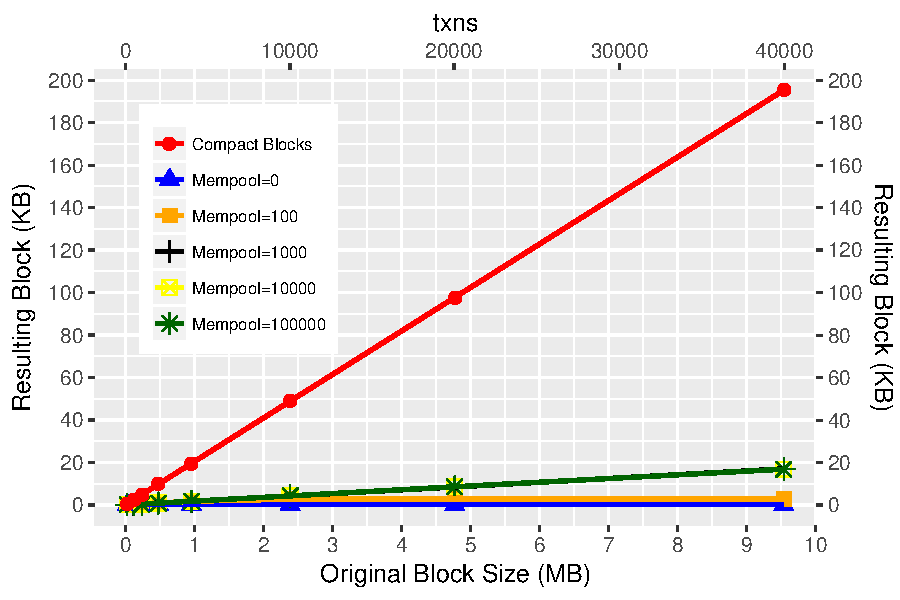
\includegraphics[width=1\textwidth]{graphs/graphene}
	\caption{A comparison of Graphene to Compact Blocks.
Mempools are expressed in terms of MB and number of transactions. Graphene is at most $1/10$th the size of Compact Blocks.  
	\label{fig:graphene}}
\end{center}\end{figure}

\para{Simulation of Bloom filters and IBLTs.}
Figure 2 shows the results of a simulation of
Compact Blocks and Graphene. The simulation is comprised
of many trials, where each trial takes as input a block size (in terms
of transactions) and the mempool size. Each protocol is executed and the
number of bytes required is recorded. Because Bloom filters
and IBLTs are probabilistic mechanisms, the simulation uses
the real data structures to ensure the accuracy of the results.
The plot is the mean of hundreds of simulations
at that point, and error bars are too small to be shown.
As the figure shows, Graphene is consistently 1/10 of the
cost of Compact Blocks or less, depending on the mempool
size. As mempool size increases, the growth of Graphene blocks to Compact Blocks is extremely slow.

%\para{Network simulation.} Next, we compare Graphene to Compact Blocks with a detailed,
%custom blockchain simulator using a Python-based discrete event simulator
%package. Our simulation models the propagation of messages across
%network links (ignoring effects from variable network bandwidth, TCP,
%etc.). Nodes accurately model any part of typical blockchain operation
%necessary for evaluating our metrics, including maintaining a mempool,
%the blockchain and its forks, and using realistic signaling.
%
%For Graphene and Compact Blocks, our simulator creates and decodes real
%Bloom filters and IBLTs, rather than merely estimating whether they
%might decode or return any false positives. If these data
%structures fail due to random chance, the nodes recover within the
%simulation. Because our simulation models detailed signaling and is written in a high-level language, our evaluations
%are based on a modest number of peers. Since our goal is a
%comparison between two choices, we expect that our results are
%representative of larger-scale scenarios.
%
%\begin{figure}[t]
% \begin{minipage}{.75\columnwidth}
% \centerline{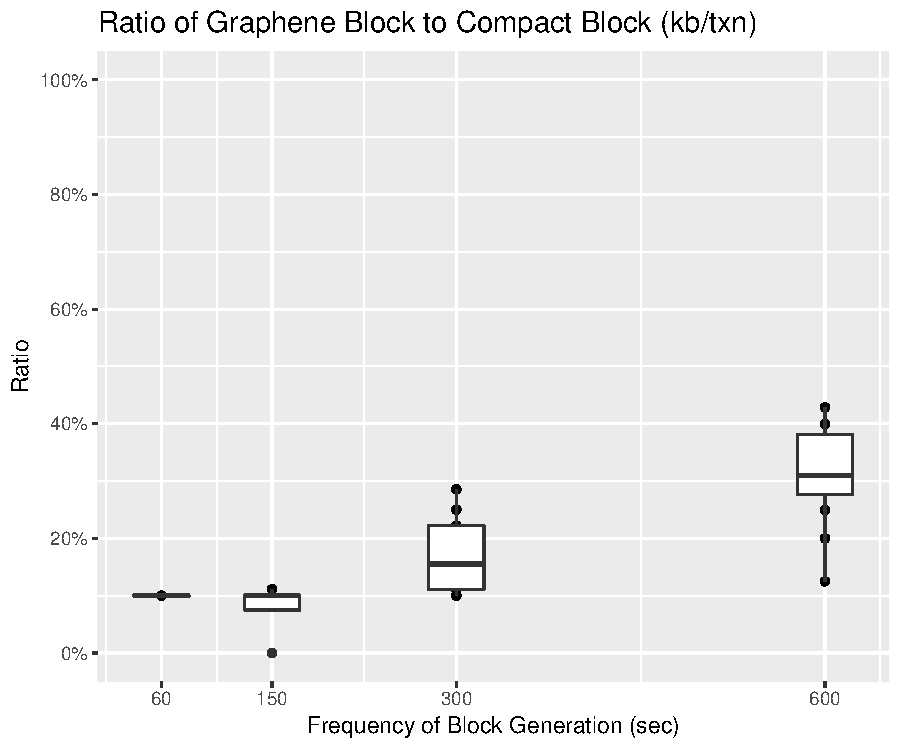
\includegraphics[width=\columnwidth]{graphs/proto}}
%\end{minipage}
%\begin{minipage}{.24\columnwidth}
%  \caption{When a random graph topology is used, Graphene reduces traffic to 60\% of the cost of Compact Blocks.}\label{fig:sim-proto}
%  \end{minipage}
%\end{figure}
%
%A challenging parameter to set is the number of transactions per
%second offered to the network by peers. Our approach is to create
%kernel density estimates (KDEs) from the transaction generation
%patterns of real world peers. To that end, we gathered data for all
%Bitcoin Core transactions during a three-month period
%%between October 27, 2015 and January 7, 2016 
%from
%{\url{http://blockchain.info}}. Each transaction in the dataset is
%labeled with an IP associated with the peer believed to have generated
%it, as well as the time it was released to the network.  For each peer,
%we normalized the release times by the time of the day in which they
%were released. We then constructed the KDE for each peer using these
%normalized transactions times and gaussian kernels with one hour
%bandwidth. The KDE for a given peer represents a probability
%distribution from which we can draw transactions over the course of a
%simulated day. For each peer in the simulator, we randomly select one
%of the KDEs corresponding to a real world peer. Because these
%distributions have been generated from real data, they are a good
%approximation of the activity of real peers over the average one-day
%interval. On the other hand, this approach is not able to model days
%of the week or seasonal phenomena in transaction creation times.
%
%Each simulation is configured to use the following parameters: 1)
%Topology: a high-degree p2p graph topology.
%%; or our {\em \tp} protocol's binary tree topology.  
%2) Block Protocol: {\em
%  Compact Blocks}; or {\em Graphene}.  3) Block capacity: 2,000
%transactions.  4) Full nodes: 50, 100, 150, or 200 peers.  In all,
% we ran 8 combinations of parameters, and we
%ran each combination with 67  different seeds;
%%20 \reminder{Update numbers} different seeds (and up to 30
%%seeds in some cases as time allowed); 
%%all told, we completed 328 (376)
%all told, we completed 536
%simulations. The seeds determined the number of transactions per
%second (by sampling our KDE, as described above), and the inter-arrival
%of transactions and blocks. 
%In all simulations, we used 6 miner
%nodes, representing 6 mining pools. Each simulation was equivalent to
%120 minutes; in sum, we simulated about 45 days of %30 days of
%blockchain operation. Blocks are generated every 2.5 minutes, like Litecoin; our results would show Graphene to have significantly greater savings if blocks were discovered every 15 seconds (like Ethereum), and show significantly smaller savings if blocks discovered were every 10 minutes (like Bitcoin). 

%On the x axis you see how often blocks are generated, and you can see that Graphene is 10% of the cost of Compact Blocks when blocks are generated every 60 seconds, so every minute. It is approximately 30% of the cost of Compact blocks, when blocks are generated every 600 seconds, or in other words, every 10 minutes. 


%Our main result is shown in
%Fig.~\ref{fig:sim-proto}, where we evaluated the total bandwidth ratio of
%Graphene to Compact Blocks, as a function of
%the number of nodes in the network. Since each run is a different
%number of KBs, we compare the ratio of an exact set of parameters
%(including the seed), varying only the protocol.  Boxplots
%show the
%distribution of results across all
%trials. Fig.~\ref{fig:sim-proto} shows that Graphene reduces traffic to  60\% of the cost of using Compact Blocks.  As the number of full nodes increases along the $x$-axis, the ratio of total traffic in the network remains steady, suggesting that our results are representative of larger networks.

%Note that gains reduce to 10\% (i.e., are 90\% of Compact Blocks) when transaction data is also included because they account for the largest portion of network traffic. However, as the number of full nodes increases along
%the $x$-axis, the ratio of total traffic in the network remains steady, suggesting that our
%results are representative of larger networks.
